\documentclass{report}
\usepackage{graphicx}
\usepackage{xcolor}
\usepackage[margin = 1in]{geometry}
\usepackage{subcaption}
\graphicspath{{../Graphs/}}


\title{Calculating the consciousness of a group of predictive markets participants}
\author{Maxime Michel - Emile Servan-Schreiber}
\date{31/07/2020} 
 
\begin{document} 
\maketitle


\chapter{Introduction}
\section{HyperMind}
\section{Goal}

The objective of this project is to build a reliability index for each market that will indicates whether it's better or not to trust its current results way before the actual results. In order to do that the idea is to compute a value representing the capacity of a group to have a 'consciousness', a value that could predict a group performance. The value is the 'integrated theory' and the group would be all the participant of a particular market. After measuring the integrated information of the market's participants we hope to see a correlation with their performance.

\chapter{Integrated Information}
\section{Definition and context}

The 'integrated information' or as we'll call it, $\phi $ , quantifies to what extend a system creates more information than the sum of its parts. Hypothetically it could reflects the global cohesion of a group. The phi metric does this by splitting the system into subsystems and then calculating how much information can be explained by looking at the system as a whole but not by looking at the subsystems separately. [1]

It was conceived to have a measurement of the consciousness of the brain but here we'll use it to try computing the 'consciousness' of a group, more particularly of a predictive market.\\

Several $\phi $ have been developed but we'll use only one, the one created by Barrett and Seth called Auto-Regressive $\phi $ [2]

\section{Auto-Regressive Phi}

\textbf{Definition of $ \phi_{AR} $} (from Barrett and Seth [2]) : $ \phi_{AR} $ compares the whole system to the sum of its parts in	terms of the log-ratio of the variance of the past state to the variance of the residual of a linear regression of the past on the present. In other words, $ \phi_{AR} $ can be understood as a measure of the extent to which the present global state of the system predicts the past global state of the system, as compared to predictions based on the most informative decomposition of the system into its component parts.\\
\\

We chose to use this particular $\phi $ thanks to Malone and Engel 's work [1], indeed they put forward that this way of computing $\phi $ is more suited for our particular case for two reasons. First we don't have enough data and too many 'nodes/users' to predict the entropies necessary to compute $\phi $. Second the other $\phi $s require an optimized partition of the 'nodes/user' that is computationally infeasible for more than 14 'nodes' and we'll have way more than that. \\


$ \phi_{AR} [X, \tau, {M_1 , M_2}] = \frac{1}{2} log\frac{det\sum X}{det\sum (E^X)} - \sum_{k=1}^{n} \frac{1}{2} log \frac{det\sum M^k}{det\sum (E^{M^k})} $ \\

$ E^{M^k}$ is the residual in $ M_{t-\tau}^k = A^{M^k} . M_t^k + E_t^{M^k} $ \\
	
$ E^{X}$ is the residual in $ X_{t-\tau} = A^{X} . X_t + E_t^X $ \\

\chapter{Data Approach}
\section{Origin of the data}

The data we used is made directly from the predictive market and put together in a .CSV format. It includes all the actions made and gather all the information about each action (date, user, type ...). This data we'll be automatically open and managed by python.\\
The csv data format creates some issues (CF Issues Encountered).

\section{Data Selection}

For the moment (This version of the project) the model doesn't need all the data offered. The current idea is to build a binary vector per individuals (participants/users) that represents who is active (exchanges values, trade) at each timestep. In a second time we'll consider the amount/price that is exchanged. In order to follow that model we are only interested in 3 categories of data, the time of the action, the user that order it and the type of action. The gathering of all those vectors constitutes a matrix for which the number of rows is the number of users and the number of columns is the number of timesteps (observation)\\

N.B. : The user 'Synt' (user id : 2) is a robot that create mirror values, therefor we excluded it directly. We also decided that the action type 'OrderCreate' or 'OrderCancel' was not an interaction and therefor can't be considered as a part of the group work, so we excluded those too.

WARNING : The data is enter chronologically in the CSV table, therefor the algorithm doesn't have to sort it, it needs to be rethink in case the data isn't sorted initially.

\section{Time scale and delay}

The question of the timestep is important because it can be at the origin of the loss of information. In this first version the chosen time step is each moment of activity. Each time there is a considered activity the algorithm open a timestep slot and register all the active users for that particular time. It works because the predictive markets ensures that the trades are as much as possible made at the same time.

The time delay is by default 1 in our work but it could have a real impact on the results so a study on its effect should be done. 

\section{Brier Score}

The brier score indicates the average error that the market does over time. Our goal is to check if this value is correlated with phi for the entire set of market accessible.

WARNING : The brier score value is written with a ',' but python can only use '.' so for the moment it needs to be changed by hand.

\chapter{Python Code}
\section{Collecting the Data}

Purpose : This file gathers all the functions made to open and arrange the data from the CSV files. Be aware that sometimes the CSV file don't have the same format, the script then needs some rearrangement (CF Issues Encountered).

\subsection{ComputeX()}

ComputeX() is made to open a CSV file that only include the data for ONE particular market. This function takes no arguments, however the 'path' of the file needs to be adapted 2 times in both lines that are like the following : \textcolor{red}{with open(r'C: ... .csv') as f:}\\
It first regroups all the information about the users and the timesteps and then it builds the matrix and return it.\\

N.B. : Be aware of the 'delimiter', by default it's a ',' but in some CSV file it can be a ';' , in this case you'll have a error (IndexError: list index out of range) . To solve that you just need to change it in both lines : \textcolor{red}{reader = csv.reader(f, delimiter = ',')}



\subsection{ManageData()}

ManageData() is practically the same as ComputeX(). It is made to open a CSV file that contains the data for SEVERAL markets. As in ComputeX() the 'path' needs to be modified and maybe the delimiter. (Cf ComputeX()).\\

This function returns 4 elements gather in a list. 
\begin{itemize}
\item The MarketList : Contains all the market IDs
\item The TimeLists : Contains a list of all the timesteps for each markets (so several list are included)
\item The UserLists : Contains a list of all the users for each markets (so several list are included)
\item MatrixList : Contains a list of each market's matrix
\end{itemize}

It's important to understand that all those 4 elements are matching, meaning that for example the tenth element of 'MarketList' matchs with the tenth of the 'TimeLists','UserList' and 'MatrixList' . (The second matrix of 'MatrixList' correspond to the second Market based on 'MarketList' ect)

\subsection{OpenMarket()}

OpenMarket() is a simple way to open a particular market included in a larger CSV file that includes several markets. This function has no arguments, it just asks the user directly. It returns the matrix associated with this chosen market. \\

N.B. : openMarket() uses ManageData(), be sure to have the right 'path' to your CSV file (the one including your particular market) in ManageData(), otherwise openMarket() won't be able to give you access to the wanted market.

\subsection{RecupError()}

RecupError() returns a list of the 'error' (Brier Score) that matchs with the 'MarketList' given by ManageData(). As in ComputeX() pay attention to the 'path' and the 'delimiter'. 

\subsection{check()}

check(X) takes a matrix as argument and check if two ligns or two columns are similar, then if it's the case it print the index of those.

\subsection{RandCcheck(X)}

RandCcheck(X) works like check() but had some noise to the similar columns or ligns so that they aren't equals afterward.

N.B. : Those two function aren't really usefull, there were made in case the similarity of columns or ligns was creating a mathematical issue, which apparently isn't the case.

\section{Correction of the Data}

Purpose : This file gather all the function that are made to make some changes on the data, like deleting some, sorting it .. before any computation or analysis is made.

\subsection{PurifierCheck()}

purifierCheck(X) takes a matrix in argument and returns duets which correspond to the number of users for each activity values. In a nutshell it gives you the number of rows with 1,2,3 ... '1'.  
It can be helpful to check the repartition. 

\subsection{PurifyProp()} 

PurifyProp(X,p) is a very important function. It takes two arguments, the matrix of data made by the functions previously presented and a variable p (for proportion) that needs to be between 0 and 1 (There is no prevention for the moment so if this condition isn't verified it will just return an error). This function erase all the 'user' (so all the rows) that are the most inactive. It delete the proportion p, chosen as argument, of the most inactive. It then return the matrix reduced from those rows.\\

It works by simply calculating the sum of '1' (which represent activity) in each row and then comparing them.

\subsection{PurifyVal()}

PurifyVal(X,v) is nearly similar to PurifyProp(). it takes to argument, the matrix and a value v that needs to a positive integer (Same as before, it will return and python error if it doesn't fit) . This function erase all 'users' (or rows) for whom the activity is under the treshold v. It then return the matrix reduced from those rows.\\

\subsection{purifyRowRandom()}

purifyRowRandom(X,prop) is a function made to randomly delete some rows of the matrix X. It delete a proportion 'prop' of all rows. It enables to observe the effect of the number of user on $\phi $.

\subsection{addColumn()}

addColumn(X,n,p) as its name indicats is made to add columns (observation) to the matrix. It takes 3 arguments, the matrix of data, n the number of columns added and p which represent the (estimated) proportion of '1' (activity) in those added column. It enables to observe the effect of the number of observation on $\phi $.

\subsection{purifyNullRow()}

purifyNullRow(X) is a function that erase all 'user' (rows) that are totally inactive, meaning composed only by '0's.

N.B. : This function is usefull because our current method is based on initially building the matrix KNOWING every user that will be a part of the market. The idea for the futur version of this project will be a 'live' evolution, meaning the programm will add the users step by step when they are active, at this moment this particular function will be useless as there will be no unactive user anymore (because the programm will not know them yet).


\section{Computing Phi}

Purpose : This file can be consider as a central piece of this work. It compute the value of phi. Those two function are largely inspired by the work of Engel and Malone [1]. It is an adaptation for our particular case. The description here will be more detailed so that a reader can adapt it again for some other use. \\

You can find the MatLab functions of Malone and Engel there (which are the models for this project's functions) : \\
Found at: doi:10.1371/journal.pcbi.1001052.s001

\subsection{reversedata()}

reversedata(X, obs, nvar) is a very simple function that just reverse the chronological order of the data in the Matrix, meaning is reverse the column order and returns the reversed matrix.

\subsection{ARphiData()}

ARphiData(X,tau) is the function were the magic is done. It takes two arguments, the data Matrix and the time delay tau (1 by default). The code is full of comments but I'll describe the process quickly here. What is important to undersand is that we work with an 'atomic' repartition, every user is a node, that is the origin of every difference with Malone and Engel's code.

\begin{itemize}
\item First the function collects nobs and nvar which are the number of column and rows. It then reverse the columns by using reversedata().
\item The mean is a constant term that isn't usefull in the regression that we'll made so we're directly remove it.
\item Then the function makes its first regression, the regression of X. changeColumn(X,Y,i) just change the column i of X in Y. The part computes the vector 'u' which gather the residuals of this regression. It finally computes the element needed for the formula, 'detResX', the determinant of the residual. The 2 following lines just compute the determinant of X.
\item Then starts the regression of every user, this is the main difference with Engel and Malone's code. This work follows an atomic partition so a regression of very user is needed. The process of the regression is the absolute same, be careful with the dimension which are very tricky. The determinants here can't be compute because the Covariances are only of one dimension, so we directly use the covariance as determinant ! 
\item All the elements are now computed, the formula can be used. Some comments are added on the code that put forward questions about some possible adaptations.The formula has been modified in order to compute the 'atomic' partition of our data. So it sums not only for two partitions as the original formula indicates but for all the rows/users/nodes.
\item The function returns phi and not Normalized phi as does the Engel and Malone function. The normalize value is only used to find the MIB, so it's not suited for our particular project.
\end{itemize}

The calculation of phi isn't always possible, in our case it's in fact often not computable. All the possible issues are listed in the chapter Issues Encountered (Inactivity Problem and Errors Type).

\section{Analyzing Phi}

Purpose : This file gather the functions useful to see the behavior of $\phi $ following various settings for a particular market. \\
N.B. : In this file you'll observe a lot of 'try-except-else', they always have the same purpose, they are made to avoid the exceptions called by ARphiData() and which cause the interruption of the computation. All those exceptions are listed in 'Issues Encountered - Errors' . This allow the function to go on even though some values of $\phi $ are not computable.

\subsection{ObsPhiVal()}

ObsPhiVal(X,n) derives from purifyVal(). It takes two arguments, the data matrix X and an integer n. This function will show the evolution of phi following the effects of purifyVal(X,v) on X, with v from 0 to n. 

\subsection{ObsPhiProp()}

ObsPhiProp(X,n) derives from purifyProp(). It takes two arguments, the data matrix X and an integer n (by default n = 98). This function will show the evolution of phi following the effects of purifyProp(X,p) on X, with p from 0.3 to n/100. 

N.B. : Those two functions are not complete as they do not avoid every exceptions . (For example if ARphiData returns 'inf' the function doesn't detect  it)

\subsection{PhiEv()}

PhiEv(X) just has the argument X but has some default variables that can be changed which are p and start (by default p = 0.6 and start = 30).This function will show the progression of $\phi $ over the market's duration. In order to do that this function computes $\phi $ for the i first columns of X, i going from start to the size of X. p is the argument of purifyProp(X,p) used in here. \\
The function print a plot, with a logarithmic scale, showing $\phi $ depending on the timestep.

\subsection{ObsZerosColumn()}

ObsZerosColumn(X) makes a plot showing the proportion of '0' in each column of the data matrix X.

\subsection{ObsPhiNodes()}

ObsPhiNodes(X) takes 1 argument but 3 other settings can be modified, it's the application of purifyRowRandom(). This function shows the effect on $\phi $ of deleting a proportion prop of the rows (chosen randomly). prop is by default between 0.1 and 0.6 (The user can modify those two values). This function uses purifyProp(x,p), p = 0.6 by default but can be modified in the code. 

\subsection{ObsPhiColumn()}

ObsPhiColumn(X) is nearly similar to ObsPhiNodes as it is the application of addColumn() and takes 1 argument. This function shows the effect on $\phi $ of adding column to X. It adds i columns, i being from 0 to 30 (30 can be changed). This function uses purifyProp(x,p), p = 0.6 by default but can be modified in the code. 

\subsection{PhiMean()}

PhiMean(X,end,p) returns the average of $\phi $s for a particular market on a certain period. In order to do that the function compute a certain amount of $\phi $s between 'start' (can be modified in the code but 0.2 by default) and 'end'. Those two variables are proportions of the total duration. p is the parameter of purifyProp(X,p) used in here. You can noticed the use of purifyNullRow(), it is very important because with our way to collect the data the matrix contains all the users initially, for that calculus of mean the not-yet active user need to be removed.

N.B.: This function used to be ver y costly in a computational point of view. In order to reduce the time of process it now includes a 'step' to limit the number of $\phi $ that are used to do the mean. This step is suit for every market but can be change if the user want so. (see 'step' in the code)

\subsection{meanWindow()}

meanWindow(X,p,s) is a function that computes $\phi $ following the 'window' method, meaning it calculates $\phi $ for the 's' last timesteps of a certain time. It does that for the whole duration of the market and returns the mean. p is the proportion of the less active user that are being ejected (argument of purifyProp(X,p)).

\section{Analyzing Markets}

Purpose : This file gather the mains functions use to analyse the markets and the power of phi by comparing it and correlating it with the brier score.

\subsection{ComputePhi()}

ComputePhi() is a very basic function that return the value of $\phi $. It doesn't take any argument, the function calls ComputeX() to collect de matrix. The user has to enter a 'treshold' which is the parameter of the function purifyProp(X,Treshold) used in here. It then simply returns the value of $\phi $.

\subsection{StudyMartket() and StudyMarkets()}

StudyMarket() and StudyMarkets() are very similar. StudyMarket() ask the user which market he wants to observe and returns the over time evolution of $\phi $ for this market and the over purification (purifyProp()) evolution of $\phi $.\\
StudyMarkets() does the same thing but, it shows the over time evolution of $\phi $ but for every market accessible by ManageData().

\subsection{StudyPhi()}

StudyPhi() is one of the most complex function of this project. It gather multiple tasks. It returns a plot showing the correlation between the Brier Score and the values of $\phi $. All the data is collected by using ManageData() and RecupError(). The function doesn't have any parameter but will ask 3 inputs to the user, a float p (proportion purified), a 'mode' of computation (Mean / Proportion / Timeste / Window) and a value 'step' (float or int depending on the chosen 'mode') There are 4 modes offers by this function :
\begin{itemize}
\item Mean : This mode will compute the mean values of $\phi $ on the segment 0.5-'step' (proportion of the market duration) for each market and then make a regression with the corresponding brier scores in order to find a correlation.
\item Prop : This mode will compute the values of $\phi $ at a certain proportion 'step' of the market's duration for each market and then make a regression with the corresponding brier scores in order to find a correlation.
\item Timestep : This mode will compute the values of $\phi $ at a certain timestep 'step' for each market and then make a regression with the corresponding brier scores in order to find a correlation.
\item Window : This mode will compute the values of $\phi $ on a 'window' meaning by considering only the 'size' (name of the variable) last timestep for each market and then make a regression with the corresponding brier scores in order to find a correlation. 'size' isn't ask to the user but can be modified in the code. (by default it's 20)
\end{itemize}

A red straight line is added representing the regression with the Correlation coefficient printed on the plot.\\
The function also return multiple data list, the BrierScore list, the Phi values List, the number of user List, the initial number of user list and the variables p and step. All those objects returns are in practice juste made for savePhiData() (the following function).



\subsection{savePhiData()}

savePhiData() is a simple function that execute StudyPhi() and save it's results in an .CSV file. By default the .CSV is saved in 'Results' bu that path can of course be modified in the function.

\subsection{BestRvalue()}

BestRvalue() is made to observe the correlation coefficient for all settings possible. It returns several plots, one for each proportion of inactive user removed (the argument of purifyProp()). For each plot the function computes the $\phi $ values for every market and computes its correlation coefficient (by regressin with the brier score as done in the previous functions) and that for every timestep ( or proportion of the duration) on a segment (modifiable in the code). By doing that it shows the evolution of this coefficient over time.\\

The settings can be modified, you'll find to loop's settings indicated by \#purification and \#step which are the set of values taken for inactivity removal and calculus of  $\phi $.\\

By default the function is only suited to follow the mode 'Timestep' of StudyPhi(), meaning the values of  $\phi $ are computed at a certain timestep. In order to observe the behavior of the correlation coefficient for  $\phi $ calculated in other modes (Mean/Window/Proportion) you'll need to copy/paste the respective part of that mode from StudyPhi(). It then only need some simple adjustments. In case of difficulty please be free to contact us.

\subsection{PhiWindow()}

PhiWindow() uses meanWindow() to compute a mean value of $\phi $ for every market and then makes a regression to try to find a correlation with the brier scores. It returns a plot and saves a CSV format with the data computed. (like savePhiData()). It doesn't take any argument but two parameters can be modified in the code, 'size' which the size of the window and 'p' as always being the proportion of users removed.

\chapter{User Guide}

In order to study $\phi $ in multiple markets the user will have to proceed to the following steps .
\begin{enumerate}
\item Change the 'path' to the CSV file containing the data in the function ManageData()
\item Change the 'path' to the CSV file containing the brier scores in the function RecupError()
\item Be aware of the parameter p of purifyProp() which is used by practically all functions (sometimes the argument is directly modifiable is the function)
\item Call StudyPhi() to compare the values of $\phi $ depending on the brier score
\item Call bestRvalue() to compare the values of the correlation coefficient for several settings
\item See for other function that can offer valuable observations
\end{enumerate}

\chapter{Issues Encountered}
\section{The Inactivity Problem}

This project is based on a binary paradigm, the user being active or not is the only thing the algorithms are sensible to. The major problem this all work had it what we call the 'inactivity problem', this issue caused the incalculability of $\phi $ in a large number of case. This issue had been noticed by Malone and Egel [1] and described by them as following [1] : 

'In some cases in our data, the AR algorithm became numerically unstable and was unable to return a value at all or returned a value that was theoretically impossible (that is, less than 0 or greater than the number of nodes/users). These problems usually occurred in cases where many nodes/users had (little or)no variance in their activities (e.g., the nodes were almost always on or almost always off, e.g. there is too many '0's).'

This justifies the necessity of using purifyProp() or purifyVal() which are made to avoid this issue by removing the less active users. However, even tough we managed to be able to compute $\phi $ most of the time by removing between 30 and 50 \% of the nodes, there is still disparities in the different markets, some of them need way more removal to return a value of  $\phi $ than others. 

\section{CSV format}

The python algorithm doesn't make sure the CSV files are correctly formated and returns an error if it's not the case. Until it's not automatized the user need to check the order of the columns, our current version needs :

\begin{itemize}
\item The time of the action : Column 1 (A in excel)
\item The UserId : Column 4 (D in excel)
\item The Type : Column 6 (F in excel)
\end{itemize}

It's the same with the Brier Score CSV, in this version :
\begin{itemize}
\item The Market ID : Column 1 (A in excel)
\item The Brier Score : Column 6 (F in excel)
\end{itemize}

All those settings can be modified, CF ManageData() and RecupError().


\section{ProcessingTime}

Some function are really long to process, maybe some estimation would be welcome. For the moment the longest is comparing all the $\phi $s by their mean (Option 'Mean' is StudyPhi()) which takes a certain time due to the number of times $\phi $ is computed. The processing time is directly linked to the size of the market. To reduce this processing time the current version simply limits the number of time $\phi $ is computed.

\section{Errors Type}

When computing Phi with ARphiData() several types of error can occur : inf, Math error, nan, 
\begin{itemize}
\item mathError: mathError is an exception released by python. It comes from the calculus of $\phi $ in ARphiData, the issue is that one of the divider in the formula is null (actually very very small). That's due to the inactivity issue. This exception is avoid by the try-except method so that it doesn't stop our functions.
\item NaN : Sometime the computed $\phi $ is 'nan' (Not a Number) that because the value is way to big or not a number. (same issue as before) The tool math.isnan() enables the functions to avoid a issue and continue to compute other values.
\item inf : Sometime the computed $\phi $ is 'inf' (for infinity). This value is of course untreatable, the tool math.isinf() enables the functions to avoid a issue and continue to compute other values.
\end{itemize}

All those errors are released by ARphiData(), they are in fact kind of the same as they have the same origin, a division by zero or a null element in the formula, this element is the determinant of X or of its regression. This comes from the inactivity problem.



\section{List instead of Arrays to make it dynamic (live)}

In this version of the project the matrix of data are made from the beginning with the data of the entire market. So from the beginning the matrix includes all the users. The idea is to make a dynamic matrix where the users are being add overtime. With the current situation everytime $\phi $ is wanted the programm creates a new matrix, it doesn't add the new data to the previous matrix. This way is more expensive and could be improved by using a dynamic matrix. (And with data $\phi $ could evolve in live)

\chapter{Results}

Our results are based on the study of 34 markets with a wide diversity of size/length. 

\section{Evolution overtime}

The first thing that is observable is that $\phi $ decrees over time, this particularity has been found in every market we tested.

\begin{figure}[ht] 
  \begin{subfigure}[b]{0.5\linewidth}
    \centering
    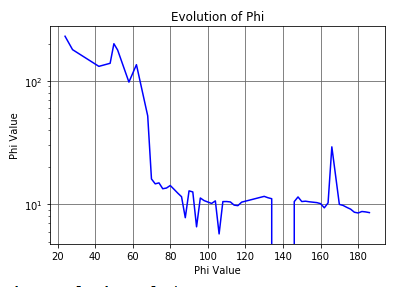
\includegraphics[width=0.75\linewidth]{./Graphs/PhiEv-Market-1416-0.5-Removed} 
    \caption{Market 1416 - 50\% Removed} 
    \label{fig1:a} 
    \vspace{4ex}
  \end{subfigure}%% 
  \begin{subfigure}[b]{0.5\linewidth}
    \centering
    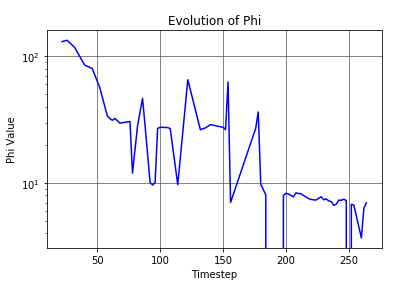
\includegraphics[width=0.75\linewidth]{./Graphs/PhiEv-Market-1443-0.5-Removed} 
    \caption{Market 1443 - 50\% Removed} 
    \label{fig1:b} 
    \vspace{4ex}
  \end{subfigure} 
  \begin{subfigure}[b]{0.5\linewidth}
    \centering
    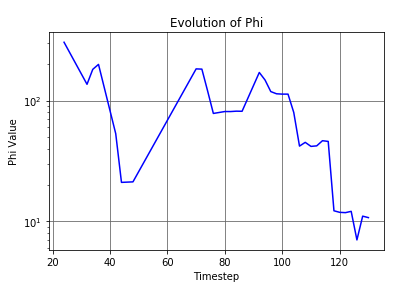
\includegraphics[width=0.75\linewidth]{./Graphs/PhiEv-Market-1413-0.4-Removed} 
    \caption{Market 1413 - 40\% Removed} 
    \label{fig1:c} 
  \end{subfigure}%%
  \begin{subfigure}[b]{0.5\linewidth}
    \centering
    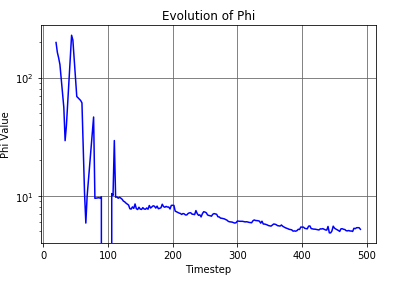
\includegraphics[width=0.75\linewidth]{./Graphs/PhiEv-Market-1439-0.4-Removed} 
    \caption{Market 1439 - 40\% Removed} 
    \label{fig1:d} 
  \end{subfigure} 
  \caption{Examples of the evolution of $\phi $ - Plots made with PhiEv()}
  \label{fi1} 
\end{figure}

This decrees was thought to be correlated with the increasing number of nodes/users over time, but ObsPhiNodes() has shown that more users equals a greater $\phi $, as shown in the following plot (Fig ). It seemed to be caused by the increasing number of observation with a relatively small amount of activity (column of a large majority of '0'). (Fig )


\begin{figure}[ht] 
  \begin{subfigure}[b]{0.5\linewidth}
    \centering
    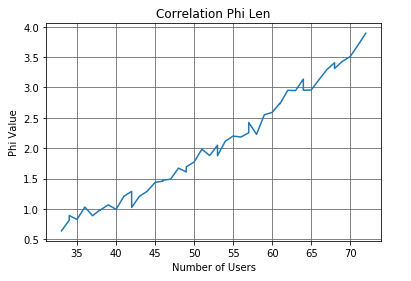
\includegraphics[width=0.75\linewidth]{./Graphs/PhiNodes-Market-1410-0.6-Removed} 
    \caption{$\phi $ as a function of the number of users }
    \label{fig2:a} 
    \vspace{4ex}
  \end{subfigure}%% 
  \begin{subfigure}[b]{0.5\linewidth}
    \centering
    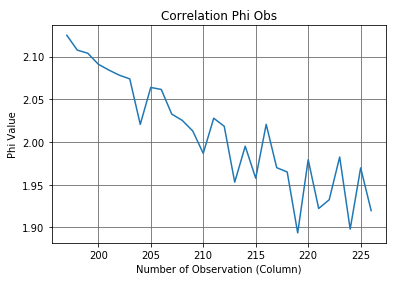
\includegraphics[width=0.75\linewidth]{./Graphs/PhiColumn-Market-1428-0.6-Removed} 
    \caption{Market 1443 - 50\% Removed} 
    \label{fig2:b} 
    \vspace{4ex}
  \end{subfigure} 
	\label{fig2}
	\caption{Plots made by ObsPhiNodes() and ObsPhiColumn()}
\end{figure}

However for $\phi $ to decrease the new observations (new timestep) needs to contain very little activity (lower than 10\% of the user active at a same timestep). It turns out that in our examples an average column has a 0.06 proportion of '1's, so it seems that the decrease of $\phi $ is simply linked to the accumulation of low activity. 

\section{Correlation with Brier Score}

The Brier score is a useful tool as it indicates the average error made by a market over time. The objective was to see a correlation between this brier score and $\phi $, which would mean a correlation between the accuracy of a groupe and the $\phi $-metric.


\chapter{Ideas of improvement}

\section{Time step andd delay}
With this scale we actually miss quite a lot of information, considering that a notable number of users participate multiple times during a same time step so we do not consider the amplitude of their activity. Maybe we could consider another scale. A way is to compare multiple timescale to see the one that correlates the best with the Brier Scores of markets.\\
\\
A real study of the effect of the time delay could also be very fructuent. We only use a value of 1 in this work but maybe some other values make more sense. (The time delay $\tau$ is a argument of ARphiData())

\section{Inactivity issue}

In this first version our way to overpass the inactivity issue has been to remove a certain proportion of the most inactive users, we used purifyProp(). However the function purifyVal() has been created but never used in the functions studying $\phi $, maybe using purifyVal() (and by that removing only the ones that are active less then one time) the results could be better.

\chapter{References}

[1] Barrett AB, Seth AK. Practical Measures of Integrated Information for Time-Series Data. Sporns O, editor. PLoS Comput Biol. 2011;7: e1001052. pmid:21283779
[2] Engel D, Malone TW (2018) Integrated information as a metric for group interaction. PLoS ONE 13(10): e0205335. https://doi.org/10.1371/journal.pone.0205335






\tableofcontents
 
\end{document}